% Created by tikzDevice version 0.12
% !TEX encoding = UTF-8 Unicode
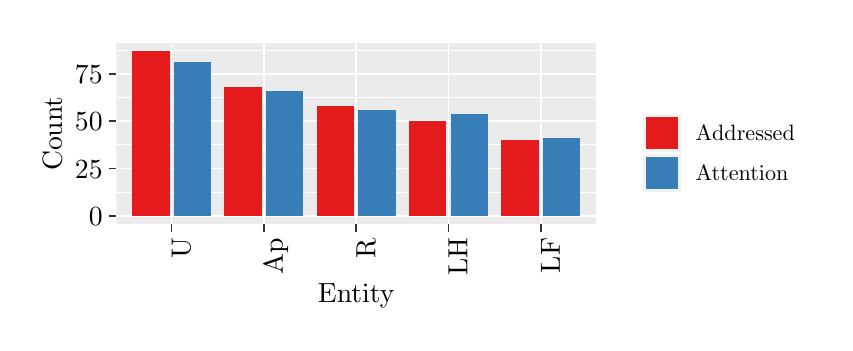
\begin{tikzpicture}[x=1pt,y=1pt]
\definecolor{fillColor}{RGB}{255,255,255}
\path[use as bounding box,fill=fillColor,fill opacity=0.00] (0,0) rectangle (288.00,106.79);
\begin{scope}
\path[clip] (  0.00,  0.00) rectangle (288.00,106.79);
\definecolor{drawColor}{RGB}{255,255,255}
\definecolor{fillColor}{RGB}{255,255,255}

\path[draw=drawColor,line width= 0.6pt,line join=round,line cap=round,fill=fillColor] (  0.00,  0.00) rectangle (288.00,106.79);
\end{scope}
\begin{scope}
\path[clip] ( 32.03, 35.78) rectangle (205.39,101.29);
\definecolor{fillColor}{gray}{0.92}

\path[fill=fillColor] ( 32.03, 35.78) rectangle (205.39,101.29);
\definecolor{drawColor}{RGB}{255,255,255}

\path[draw=drawColor,line width= 0.3pt,line join=round] ( 32.03, 47.31) --
	(205.39, 47.31);

\path[draw=drawColor,line width= 0.3pt,line join=round] ( 32.03, 64.43) --
	(205.39, 64.43);

\path[draw=drawColor,line width= 0.3pt,line join=round] ( 32.03, 81.54) --
	(205.39, 81.54);

\path[draw=drawColor,line width= 0.3pt,line join=round] ( 32.03, 98.65) --
	(205.39, 98.65);

\path[draw=drawColor,line width= 0.6pt,line join=round] ( 32.03, 38.76) --
	(205.39, 38.76);

\path[draw=drawColor,line width= 0.6pt,line join=round] ( 32.03, 55.87) --
	(205.39, 55.87);

\path[draw=drawColor,line width= 0.6pt,line join=round] ( 32.03, 72.98) --
	(205.39, 72.98);

\path[draw=drawColor,line width= 0.6pt,line join=round] ( 32.03, 90.10) --
	(205.39, 90.10);

\path[draw=drawColor,line width= 0.6pt,line join=round] ( 52.03, 35.78) --
	( 52.03,101.29);

\path[draw=drawColor,line width= 0.6pt,line join=round] ( 85.37, 35.78) --
	( 85.37,101.29);

\path[draw=drawColor,line width= 0.6pt,line join=round] (118.71, 35.78) --
	(118.71,101.29);

\path[draw=drawColor,line width= 0.6pt,line join=round] (152.05, 35.78) --
	(152.05,101.29);

\path[draw=drawColor,line width= 0.6pt,line join=round] (185.38, 35.78) --
	(185.38,101.29);
\definecolor{fillColor}{RGB}{228,26,28}

\path[fill=fillColor] ( 37.78, 38.76) rectangle ( 51.28, 98.31);
\definecolor{fillColor}{RGB}{55,126,184}

\path[fill=fillColor] ( 52.78, 38.76) rectangle ( 66.28, 94.21);
\definecolor{fillColor}{RGB}{228,26,28}

\path[fill=fillColor] ( 71.12, 38.76) rectangle ( 84.62, 85.31);
\definecolor{fillColor}{RGB}{55,126,184}

\path[fill=fillColor] ( 86.12, 38.76) rectangle ( 99.62, 83.94);
\definecolor{fillColor}{RGB}{228,26,28}

\path[fill=fillColor] (104.46, 38.76) rectangle (117.96, 78.46);
\definecolor{fillColor}{RGB}{55,126,184}

\path[fill=fillColor] (119.46, 38.76) rectangle (132.96, 77.09);
\definecolor{fillColor}{RGB}{228,26,28}

\path[fill=fillColor] (137.79, 38.76) rectangle (151.30, 72.98);
\definecolor{fillColor}{RGB}{55,126,184}

\path[fill=fillColor] (152.80, 38.76) rectangle (166.30, 75.72);
\definecolor{fillColor}{RGB}{228,26,28}

\path[fill=fillColor] (171.13, 38.76) rectangle (184.63, 66.14);
\definecolor{fillColor}{RGB}{55,126,184}

\path[fill=fillColor] (186.14, 38.76) rectangle (199.64, 66.82);
\end{scope}
\begin{scope}
\path[clip] (  0.00,  0.00) rectangle (288.00,106.79);
\definecolor{drawColor}{RGB}{0,0,0}

\node[text=drawColor,anchor=base east,inner sep=0pt, outer sep=0pt, scale=  1.00] at ( 27.08, 35.31) {0};

\node[text=drawColor,anchor=base east,inner sep=0pt, outer sep=0pt, scale=  1.00] at ( 27.08, 52.43) {25};

\node[text=drawColor,anchor=base east,inner sep=0pt, outer sep=0pt, scale=  1.00] at ( 27.08, 69.54) {50};

\node[text=drawColor,anchor=base east,inner sep=0pt, outer sep=0pt, scale=  1.00] at ( 27.08, 86.65) {75};
\end{scope}
\begin{scope}
\path[clip] (  0.00,  0.00) rectangle (288.00,106.79);
\definecolor{drawColor}{gray}{0.20}

\path[draw=drawColor,line width= 0.6pt,line join=round] ( 29.28, 38.76) --
	( 32.03, 38.76);

\path[draw=drawColor,line width= 0.6pt,line join=round] ( 29.28, 55.87) --
	( 32.03, 55.87);

\path[draw=drawColor,line width= 0.6pt,line join=round] ( 29.28, 72.98) --
	( 32.03, 72.98);

\path[draw=drawColor,line width= 0.6pt,line join=round] ( 29.28, 90.10) --
	( 32.03, 90.10);
\end{scope}
\begin{scope}
\path[clip] (  0.00,  0.00) rectangle (288.00,106.79);
\definecolor{drawColor}{gray}{0.20}

\path[draw=drawColor,line width= 0.6pt,line join=round] ( 52.03, 33.03) --
	( 52.03, 35.78);

\path[draw=drawColor,line width= 0.6pt,line join=round] ( 85.37, 33.03) --
	( 85.37, 35.78);

\path[draw=drawColor,line width= 0.6pt,line join=round] (118.71, 33.03) --
	(118.71, 35.78);

\path[draw=drawColor,line width= 0.6pt,line join=round] (152.05, 33.03) --
	(152.05, 35.78);

\path[draw=drawColor,line width= 0.6pt,line join=round] (185.38, 33.03) --
	(185.38, 35.78);
\end{scope}
\begin{scope}
\path[clip] (  0.00,  0.00) rectangle (288.00,106.79);
\definecolor{drawColor}{RGB}{0,0,0}

\node[text=drawColor,rotate= 90.00,anchor=base east,inner sep=0pt, outer sep=0pt, scale=  1.00] at ( 58.92, 30.83) {U};

\node[text=drawColor,rotate= 90.00,anchor=base east,inner sep=0pt, outer sep=0pt, scale=  1.00] at ( 92.26, 30.83) {Ap};

\node[text=drawColor,rotate= 90.00,anchor=base east,inner sep=0pt, outer sep=0pt, scale=  1.00] at (125.60, 30.83) {R};

\node[text=drawColor,rotate= 90.00,anchor=base east,inner sep=0pt, outer sep=0pt, scale=  1.00] at (158.93, 30.83) {LH};

\node[text=drawColor,rotate= 90.00,anchor=base east,inner sep=0pt, outer sep=0pt, scale=  1.00] at (192.27, 30.83) {LF};
\end{scope}
\begin{scope}
\path[clip] (  0.00,  0.00) rectangle (288.00,106.79);
\definecolor{drawColor}{RGB}{0,0,0}

\node[text=drawColor,anchor=base,inner sep=0pt, outer sep=0pt, scale=  1.00] at (118.71,  7.44) {Entity};
\end{scope}
\begin{scope}
\path[clip] (  0.00,  0.00) rectangle (288.00,106.79);
\definecolor{drawColor}{RGB}{0,0,0}

\node[text=drawColor,rotate= 90.00,anchor=base,inner sep=0pt, outer sep=0pt, scale=  1.00] at ( 12.39, 68.53) {Count};
\end{scope}
\begin{scope}
\path[clip] (  0.00,  0.00) rectangle (288.00,106.79);
\definecolor{fillColor}{RGB}{255,255,255}

\path[fill=fillColor] (216.39, 41.66) rectangle (282.50, 95.40);
\end{scope}
\begin{scope}
\path[clip] (  0.00,  0.00) rectangle (288.00,106.79);
\definecolor{drawColor}{RGB}{255,255,255}
\definecolor{fillColor}{gray}{0.95}

\path[draw=drawColor,line width= 0.6pt,line join=round,line cap=round,fill=fillColor] (221.89, 61.62) rectangle (236.34, 76.07);
\end{scope}
\begin{scope}
\path[clip] (  0.00,  0.00) rectangle (288.00,106.79);
\definecolor{fillColor}{RGB}{228,26,28}

\path[fill=fillColor] (223.31, 63.04) rectangle (234.92, 74.65);
\end{scope}
\begin{scope}
\path[clip] (  0.00,  0.00) rectangle (288.00,106.79);
\definecolor{drawColor}{RGB}{255,255,255}
\definecolor{fillColor}{gray}{0.95}

\path[draw=drawColor,line width= 0.6pt,line join=round,line cap=round,fill=fillColor] (221.89, 47.16) rectangle (236.34, 61.62);
\end{scope}
\begin{scope}
\path[clip] (  0.00,  0.00) rectangle (288.00,106.79);
\definecolor{fillColor}{RGB}{55,126,184}

\path[fill=fillColor] (223.31, 48.59) rectangle (234.92, 60.20);
\end{scope}
\begin{scope}
\path[clip] (  0.00,  0.00) rectangle (288.00,106.79);
\definecolor{drawColor}{RGB}{0,0,0}

\node[text=drawColor,anchor=base west,inner sep=0pt, outer sep=0pt, scale=  0.80] at (241.34, 66.09) {Addressed};
\end{scope}
\begin{scope}
\path[clip] (  0.00,  0.00) rectangle (288.00,106.79);
\definecolor{drawColor}{RGB}{0,0,0}

\node[text=drawColor,anchor=base west,inner sep=0pt, outer sep=0pt, scale=  0.80] at (241.34, 51.64) {Attention};
\end{scope}
\end{tikzpicture}
